\section{DP Minimum Vertex Cover for \repair\ }\label{sec:vertex_cover}


% This section also computes the optimal repair measure 
% $\repair$ using the conflict graph. The optimal repair measure over $D$ is equivalent to the minimum number of vertices that need to be repaired (or removed) such that there are no more conflicts in the dataset. For the conflict graph $\graph$, the $\repair$ measure can be formulated as calculating the minimum vertex cover size of $\graph$. However, calculating minimum vertex cover is an NP-hard problem. Therefore, our work uses the well-known polynomial time algorithm for computing vertex cover that guarantees a 2-approximation ratio~\cite{vazirani1997approximation}. This algorithm is a randomized algorithm that goes through a random ordering of the edges. For each edge, if the two nodes connecting it have not been encountered before, it adds both nodes to the vertex-cover set and removes all edges of those nodes from the edge list. The algorithm continues until the edge list is empty. 
This section details our approach for computing the optimal repair measure, $\repair$, using the conflict graph. \repair\ is defined as the minimum number of vertices that must be removed to eliminate all conflicts within the dataset. For the conflict graph $\graph$, this corresponds to finding the minimum vertex cover -- an NP-hard problem. To address this, we apply a well-known polynomial-time algorithm that provides a 2-approximation for vertex cover~\cite{vazirani1997approximation}. This randomized algorithm iterates through a random ordering of edges, adding both nodes of each edge to the vertex cover if they haven't been encountered, then removes all incident edges. The process repeats until the edge list is exhausted. 
In our setting, we aim to compute the minimum vertex cover size while satisfying DP. A straightforward approach would be to analyze the sensitivity of the 2-approximation algorithm and add the appropriate DP noise. However, determining the sensitivity of this naive approximation is challenging, as the algorithm's output can fluctuate significantly depending on the order of selected edges. This variability is illustrated in \Cref{example:naive_vertexcover}.

% Algorithm~\ref{algo:naive_vertexcover} illustrates the approximation algorithm. Line 1 starts by first initializing two variables to store the vertex cover, $C$, and its size, $c$. In lines 2-5, the algorithm randomly chooses an edge $e(u,v)$ from the graph, removes all other edges in the list connected to either $u$ or $v$ and appends both vertices $u$ and $v$ to the vertex cover $C$ and its size by $2$. 

% We are interested in computing the minimum vertex cover size with DP in our setting. One way to do so is to analyze the sensitivity of the 2-approximation algorithm and add DP noise to the output size of the vertex cover. However, we note that it is hard to calculate the sensitivity of the naive approximation algorithm as the output of the algorithm may vary drastically based on the order of the selected edges. We illustrate this issue in Example~\ref{example:naive_vertexcover}.


% \begin{algorithm}
% \caption{2-Approximation Vertex Cover}
% \label{algo:naive_vertexcover}
%     \KwData{Graph $\mathcal{G} (V,E)$}
%     \KwResult{Vertex cover size $c$}
%     Initialize vertex cover set $C = \emptyset$ and size $c=0$\;
%     \While{E $\neq \emptyset$} {
%     randomly pick edge $e\{u, v\}$ from E\;
%     remove all edges in $E$ incident to $u$ and $v$\;
%     add $u$ and $v$ to $C$ and $c = c + 2$\;
%     }
%     return $c$\;
% \end{algorithm}


\begin{figure}
    \begin{center}
    \scalebox{1.0}{
    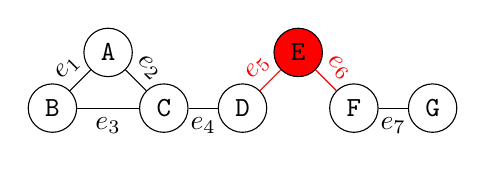
\begin{tikzpicture}[main/.style = {draw, circle}]
        % nodes
        \node[main] (1) {{\tt B}}; 
        \node[main] (2) [above right of=1] {{\tt A}};
        \node[main] (3) [below right of=2] {{\tt C}};
        \node[main] (4) [right of=3] {{\tt D}};
        \node[main, fill=red] (5) [above right of=4] {{\tt E}};
        \node[main] (6) [below right of=5] {{\tt F}};
        \node[main] (7) [right of=6] {{\tt G}};
        % edges
        \draw (1) -- node[midway, above, sloped]{$e_1$} (2);
        \draw (2) -- node[midway, above, sloped]{$e_2$} (3);
        \draw (1) -- node[midway, below, sloped]{$e_3$} (3);
        \draw (3) -- node[midway, below, sloped]{$e_4$}(4);
        \draw[red] (5) -- node[midway, above, sloped]{$e_6$}(6);
        \draw[red] (4) --  node[midway, above, sloped]{$e_5$}(5);
        \draw (6) -- node[midway, below, sloped]{$e_7$}(7);
    \end{tikzpicture} 
    }
\end{center}
\caption{Toy graph example $\mathcal{G}$ with seven nodes ({\tt A} to {\tt G}) and seven edges. Consider a neighboring graph $\mathcal{G}'$ with the differing node {\tt E} (red) and its two edges. }
\label{fig:examplegraph}
\end{figure}

\begin{example}
Let us consider a graph $\mathcal{G}$ with 7 vertices {\tt A} to {\tt G} and 7 edges $e_1$ to $e_7$ as shown in Figure~\ref{fig:examplegraph}. We can have a neighboring graph $\mathcal{G}'$ by considering the vertex {\tt E} as the differing vertex and two of its edges $e_5$ and $e_6$ as the differing edges. This example shows that according to the vanilla 2-approximate algorithm, the output for the graphs $\mathcal{G}$ and $\mathcal{G}'$ may vary drastically. For $\mathcal{G}$, if $e_2$ is selected followed by $e_7$, then the vertex cover size is 4. However, for graph $\mathcal{G}'$, if $e_1$ or $e_4$ is selected first and subsequently after the other one $e_6$ is selected, then the output is 6. Moreover, this difference may get significantly large if the above graph is stacked multiple times and the corresponding vertex that creates this difference is chosen every time. 
\label{example:naive_vertexcover}
\end{example}




\begin{algorithm}[t]
\caption{DP approximation of minimum vertex cover size for $\repair$}
\label{algo:dp_vertexcover}
    \KwData{Graph $\mathcal{G} (V,E)$, stable global ordering $\Lambda$, privacy parameter $\epsilon$}
    \KwResult{DP minimum vertex cover size for $\repair$}
    Initialize vertex cover set $C = \emptyset$ and size $c = 0$ \\
    Initialize edge list $E_0 = E$ \\
    \For{$i \in \{1 \dots |\Lambda|\}$}{
        pop edge $e_i = \{u, v\}$ in order from $\Lambda$\\
        add $u$ and $v$ to $C$ and $c = c + 2$\\
        $E_{i+1}$ = remove all edges incident to $u$ or $v$ from $E_i$\\    
    }
    {\bf Return} $c$\ + Lap($\epsilon$/2)
\end{algorithm}

% We note that the analysis of the algorithm gets complicated because of the random order of the selection of edges. 
% Therefore, inspired by Day et al.~\cite{day2016publishing}, we make a minor change in the algorithm by traversing the edges in a particular order. We use a similar stable ordering $\Lambda$ defined in Section~\ref{sec:prelim-dp}. The updated algorithm is shown in Algorithm~\ref{algo:dp_vertexcover}. We start by initializing an empty vertex cover set $C$ and its size $c$. We then start an iteration over all edges in the same ordering as the stable ordering $\Lambda$. For each edge $e_i = {u,v} \in E$ that is part of the graph, we add both $u$ and $v$ to $C$ and correspondingly increment the size $c$. We also remove all other edges including $e_i$ that are connected to $u$ or $v$ from $E$ and continue the iteration. The sensitivity of this algorithm is given by \cref{prop:vertexcover_sens}. 
To solve the sensitivity issue, we make a minor change in the algorithm by traversing the edges in a particular order (drawing on~\cite{day2016publishing}). We use a similar stable ordering $\Lambda$ defined in \Cref{sec:prelim-dp}. The new algorithm is shown in Algorithm~\ref{algo:dp_vertexcover}. We initialize an empty vertex cover set $C$, its size $c$, and an edge list (lines 1--2). We then start an iteration over all edges in the same ordering as the stable ordering $\Lambda$ (line 3). For each edge $e_i = \{u,v\} \in E$ that is part of the graph, we add both $u$ and $v$ to $C$ and correspondingly increment the size $c$ (lines 4--5). We remove all other edges, including $e_i$, connected to $u$ or $v$ from $E$ and continue the iteration (line 5). Finally, we return the noisy size of the vertex cover (line 6). The sensitivity of this algorithm is given by \cref{prop:vertexcover_sens}. 




\begin{proposition}\label{prop:vertexcover_sens}
Algorithm~\ref{algo:dp_vertexcover} obtains a vertex cover, and its size has a sensitivity of 2.
    % For any two neighboring graphs $\mathcal{G} \neighbor \mathcal{G}^\prime$ that differ by one node, we have
    % \begin{equation*}
    %     \|c - c' \| \leq 2 
    % \end{equation*},
    % where $c$ and $c'$ are the vertex cover sizes of $\mathcal{G}$ and $\mathcal{G}'$ obtained from Algorithm~\ref{algo:dp_vertexcover} respectively.
\end{proposition}



\ifpaper
\begin{proof} (sketch)
Consider two graphs that differ by one node $v^*$ and the edges connected to it. The stable ordering of edges $\Lambda$ in algorithm~\ref{algo:dp_vertexcover} restricts the order in which the edges occur in both graphs. As the algorithm removes all edges of a particular node once observed, we can delineate 3 cases depending on which of the two graphs has the differing node. This allows us to show proof by induction. The detailed proof is in the full version~\cite{full_paper}.
\end{proof}
%Due to space constraints, we defer this proof to the full paper \ag{Add citation when available}. 

\else
The proof can be found in ~\cref{app:vertext_cover_sensitivity}.
\eat{
\proof
Let's assume without loss of generality that
$\mathcal{G}^{\prime}=\left(V^{\prime}, E^{\prime}\right)$ has an additional node $v^{+}$compared to $\mathcal{G}=$ $(V, E)$, i.e., $V^{\prime}=V \cup\left\{v^{+}\right\}, E^{\prime}=E \cup E^{+}$, and $E^{+}$ is the set of all edges incident to $v^{+}$ in $\mathcal{G}^{\prime}$. We prove the theorem using a mathematical induction on $i$ that iterates over all edges of the global stable ordering $\Lambda$.

\underline{Base}: At step 0, the value of $c$ and $c'$ are both 0.

\underline{Hypothesis}: As the algorithm progresses at each step $i$ when the edge $e_i$ is chosen, either the edges of graph $\mathcal{G}'$ which is denoted by $E'_i$ has an extra vertex or the edge of graph $\mathcal{G}$ has an extra vertex. Thus, we can have two cases depending on some node $v^*$ and its edges $\{v^*\}$. Note that at the beginning of the algorithm, $v^*$ is the differing node $v^+$ and $\mathcal{G}'$ has the extra edges of $v^*/v^+$, but $v^*$ may change as the algorithm progresses. The cases are as illustrated below:
\begin{itemize}
    \item Case 1: $E_i$ does not contain any edges incident to $v^*$, $E'_i = E_i + \{ v^* \}$ and the vertex cover sizes at step $i$ could be $c_i = c'_i$ or $c_i = c'_i + 2$.
    \item Case 2: $E'_i$ does not contain any edges incident to $v^*$, $E_i = E'_i + \{ v^* \}$ and the vertex cover sizes at step $i$ could be $c_i = c'_i$ or $c'_i = c_i + 2$.
    \item Case 3: $E_i=E'_i$ and the vertex cover sizes at step $i$ is $c_i = c'_i$. This case occurs only when the additional node $v^+$ has no edges. 
\end{itemize}


\begin{figure*}
    \begin{subfigure}[b]{\textwidth}
    \centering
    \includegraphics[width=0.19\textwidth]{images/true_vs_private/truevsprivate_Stock_positive_degree_nodes_samegraph_10000_rnoise_eps_1.0.jpg}
    \hfill
    \includegraphics[width=0.19\textwidth]{images/true_vs_private/truevsprivate_Tax_positive_degree_nodes_samegraph_10000_rnoise_eps_1.0.jpg}
    \hfill
    \includegraphics[width=0.19\textwidth]{images/true_vs_private/truevsprivate_Hospital_positive_degree_nodes_samegraph_10000_rnoise_eps_1.0.jpg}
    \hfill
    \includegraphics[width=0.19\textwidth]{images/true_vs_private/truevsprivate_Flight_positive_degree_nodes_samegraph_10000_rnoise_eps_1.0.jpg}
    \hfill
    \includegraphics[width=0.19\textwidth]{images/true_vs_private/truevsprivate_Adult_positive_degree_nodes_samegraph_10000_rnoise_eps_1.0.jpg}
    \includegraphics[width=0.2\textwidth]{images/legend_2.png}
    \caption{$\problematic$ (Positive degree nodes)}
    \label{fig:tp_rnoise_pdedges}
    \end{subfigure}
    \begin{subfigure}[b]{\textwidth}
    \centering
    \includegraphics[width=0.19\textwidth]{images/true_vs_private/truevsprivate_Stock_no_of_edges_samegraph_10000_rnoise_eps_1.0_r2t.jpg}
    \hfill
    \includegraphics[width=0.19\textwidth]{images/true_vs_private/truevsprivate_Tax_no_of_edges_samegraph_10000_rnoise_eps_1.0_r2t.jpg}
    \hfill
    \includegraphics[width=0.19\textwidth]{images/true_vs_private/truevsprivate_Hospital_no_of_edges_samegraph_10000_rnoise_eps_1.0_r2t.jpg}
    \hfill
    \includegraphics[width=0.19\textwidth]{images/true_vs_private/truevsprivate_Flight_no_of_edges_samegraph_10000_rnoise_eps_1.0_r2t.jpg}
    \hfill
    \includegraphics[width=0.19\textwidth]{images/true_vs_private/truevsprivate_Adult_no_of_edges_samegraph_10000_rnoise_eps_1.0_r2t.jpg}
    \includegraphics[width=0.3\textwidth]{images/legend2_r2t.png}
    \caption{$\mininconsistency$ (Number of edges)}
    \label{fig:tp_rnoise_nedges}
    \end{subfigure}
      \begin{subfigure}[b]{\textwidth}
         \centering
         \includegraphics[width=0.19\textwidth]{images/true_vs_private/truevsprivate_Stock_vertex_cover_samegraph_10000_rnoise_eps_1.0.jpg}
         \hfill
         \includegraphics[width=0.19\textwidth]{images/true_vs_private/truevsprivate_Tax_vertex_cover_samegraph_10000_rnoise_eps_1.0.jpg}
         \hfill
         \includegraphics[width=0.19\textwidth]{images/true_vs_private/truevsprivate_Hospital_vertex_cover_samegraph_10000_rnoise_eps_1.0.jpg}
         \hfill
         \includegraphics[width=0.19\textwidth]{images/true_vs_private/truevsprivate_Flight_vertex_cover_samegraph_10000_rnoise_eps_1.0.jpg}
         \hfill
         \includegraphics[width=0.19\textwidth]{images/true_vs_private/truevsprivate_Adult_vertex_cover_samegraph_10000_rnoise_eps_1.0.jpg}
         \includegraphics[width=0.2\textwidth]{images/legend_2.png}
         \caption{$\repair$ (Size of vertex cover)}
         \label{fig:tp_rnoise_vcover}
     \end{subfigure}
     \caption{True vs Private estimates for all dataset with RNoise $\alpha = 0.01$ at $\epsilon=1$. The $\problematic$ measure (figure a) and $\mininconsistency$ measure (figure b) are computed using our graph projection approach, and $\repair$ measure using our private vertex cover size approach. }
     \label{fig:tp_RNoise}
\end{figure*}



\underline{Induction}: At step $i+1$, lets assume an edge $e_{i+1} = \{u, v\}$ is chosen. Depending on the $i^{th}$ step, we can have 2 cases as stated in the hypothesis.

\begin{itemize}
    \item Case 1 (When $E'_i$ has the extra edges of $v^*$): We can have the following subcases at step $i+1$ depending on $e_{i+1}$.
        \begin{enumerate}[label=\alph*),ref=\alph*]
            \item If the edge is part of $E'_{i}$ but not of $E_i$ ($e_{i+1} \in E'_{i} \setminus E_{i}$): Then $e_{i+1} = \{u, v\}$ should not exist in $E_i$ (according to the hypothesis at the $i$ step) and one of $u$ or $v$ must be $v^*$. Let's assume without loss of generality that $v$ is $v^*$. The algorithm will add $(u, v)$ to $C'$ and update $c'_{i+1} = c_i + 2$. Hence, we have either $c'_{i+1} = c_{i+1}$ or $c'_{i+1} = c + 2$.

            In addition, all edges of $u$ and $v/v^*$ will be removed from $E'_{i+1}$. Thus, we have $E_{i+1} = E'_{i+1} + \{u\}$, where $\{u\}$ represent edges of $u$. Now $u$ becomes the new $v^*$ and moves to Case 2 for the $i+1$ step.  
            
            \item If the edge is part of both $E'_i$ and $E_i$($e_{i+1} \in E'_i$ and $e_{i+1} \in E_i$): In this case $(u,v)$ will be added to both $C$ and $C'$ and the vertex sizes with be updated as $c_{i+1} = c_i + 2$ and $c'_{i+1} = c' + 2$. 

            Also, the edges adjacent to $u$ and $v$ will be removed from $E_i$ and $E'_i$. We still have $E'_i = E + {v^*}$ (the extra edges of $v^*$ and remain in case 1 for step i+1. 

            \item If the edge is part of neither $E'_i$ nor $E_i$ (If $e_{i+1} \in E'_i$ and $e_{i+1} \in E_i$): the algorithm makes no change. The previous state keep constant: $E'_{i+1} = E'_i, E_{i+1} = E_i$ and $c'_{i+1} = c'_i, c_{i+1} = c_i$. The extra edges of $v^*$ are still in $E'_{i+1}$.
        \end{enumerate}
        
    \item Case 2 (When $E_i$ has the extra edges of $v^*$) : This case is symmetrical to Case 1. There will be three subcases similar to Case 1 -- a) in which after the update, the state of the algorithm switches to Case 1, b) in which the state remains in Case 2, and c) where no update takes place.  

    \item Case 3 (When $E_i = E'_i$): In this case, the algorithm progresses similarly for both the graphs, and remains in case 3 with equal vertex covers, $c_{i+1} = c'_{i+1}$.
\end{itemize}

Our induction proves that our hypothesis is true. The algorithm starts with Case 1, either in the same case or oscillates between Case 1 and Case 2. Hence, as per our hypothesis statement, the difference between the vertex cover sizes is upper-bounded by 2.
\qed
}
\fi



\begin{example}
    Let us consider our running example in Figure~\ref{fig:examplegraph} as input to Algorithm~\ref{algo:dp_vertexcover} and use it to understand the proof. We have two graphs -- $\mathcal{G}$ which has $6$ vertices $V = [{\tt A, B, C, D, F, G}]$ and edges $E = [e_1, e_2, e_3, e_4, e_7]$ and $\mathcal{G}'$ has $7$ vertices $V' = [{\tt A, B, C, D, E, F, G}]$ and edges $E' = [e_1, e_2, \dots, e_7]$. The total possible number of edges is $\binom{7}{2} = 21$, and we can have a global stable ordering of the edges $\Lambda$ depending on the lexicographical ordering of the vertices as $e_1, e_2, e_3, \dots, e_{21}$. When the algorithm starts, both vertex cover sizes are initialized to $c=0, c'=0$, and the algorithm's state is in Case 1 with $v^* = {\tt E}$. We delineate the next steps of the algorithm below:
    \begin{itemize*}
        \item Iteration 1 (Subcase 1b) : $e_1 ({\tt A,B})$ is chosen. {\tt A} and {\tt B} are both in $E_0$ and $E'_0$. Hence $c = 2, c'= 2$.
        \item Iteration 2, 3 (Subcase 1c) : $e_2 ({\tt A,C})$ and $e_3 ({\tt B,C})$ are chosen. Both are removed in iteration 1. Hence $c = 2, c'= 2$.
        \item Iteration 4 (Subcase 1b) : $e_4 ({\tt C, D})$ is chosen. {\tt C} and {\tt D} are both in $E_3$ and $E'_3$. Hence $c = 4, c'= 4$.
        \item Iteration 5 (Subcase 1c) : $e_5 ({\tt D,E})$ is chosen, removed from $E'_4$ in Iteration 4, and was never present in $E$. Hence $c = 4, c'= 4$.
        \item Iteration 6 (Subcase 1a) : $e_6 ({\tt E, F})$ is chosen. It is in $E'_5$ but not in $E_5$. Hence, $c = 4, c'= 6$ and the new $v^* = {\tt E}$.
        \item Iteration 7 (Subcase 2a) : $e_7 ({\tt F,G})$ is chosen. It is in $E_6$ but removed from $E_6$ in Iteration 6. Hence, $c = 6, c'= 6$, and the algorithm is complete.
    \end{itemize*}
\end{example}





\paratitle{Privacy and utility analysis}
We now show the privacy and utility analysis of Algorithm~\ref{algo:dp_vertexcover} using Theorem~\ref{thm:vertex_cover_priv_util_analysis} below.

\begin{theorem}~\label{thm:vertex_cover_priv_util_analysis}
    % Algorithm~\ref{algo:dp_vertexcover} satisfies $\epsilon$-node DP and always outputs the size of a 2-approximate vertex cover of graph $\mathcal{G}$.
    \reva{Algorithm~\ref{algo:dp_vertexcover} satisfies $\epsilon$-node DP and, prior to adding noise in line 7, obtains a 2-approximation vertex cover size.} 
    % of the graph $\mathcal{G}$.}
\end{theorem}

\begin{proof}
The Algorithm~\ref{algo:dp_vertexcover} satisfies $\epsilon$-node DP as we calculate the private vertex cover using the Laplace mechanism with sensitivity $2$ according to Proposition~\ref{prop:vertexcover_sens}. It is also a 2-approximation as the stable ordering $\Lambda$ in Algorithm~\ref{algo:dp_vertexcover} can be perceived as one particular random order of the edges and hence has the same utility as the original 2-approximation algorithm. 
\end{proof}
